\documentclass[11pt,fleqn, openany]{book} % Default font size and left-justified equations

%%%%%%%%%%%%%%%%%%%%%%%%%%%%%%%%%%%%%%%%%
% The Legrand Orange Book
% Structural Definitions File
% Version 2.1 (26/09/2018)
%
% Original author:
% Mathias Legrand (legrand.mathias@gmail.com) with modifications by:
% Vel (vel@latextemplates.com)
% 
% This file was downloaded from:
% http://www.LaTeXTemplates.com
%
% License:
% CC BY-NC-SA 3.0 (http://creativecommons.org/licenses/by-nc-sa/3.0/)
%
%%%%%%%%%%%%%%%%%%%%%%%%%%%%%%%%%%%%%%%%%

%----------------------------------------------------------------------------------------
%	VARIOUS REQUIRED PACKAGES AND CONFIGURATIONS
%----------------------------------------------------------------------------------------

\usepackage[table]{xcolor}

\usepackage{graphicx}
\usepackage{tabularx} % Required for including pictures
\usepackage{pgf,tikz,tkz-tab,eurosym,yhmath, stmaryrd}
\usepackage{pgfplots}
\usepackage{mathrsfs}
\usetikzlibrary{patterns}
\usetikzlibrary{trees}
\graphicspath{{../../Pictures/}}
\usepackage{multicol} 


\usepackage[english]{babel} % English language/hyphenation
\usepackage{icomma}
\usepackage{enumitem} % Customize lists
\setlist{nolistsep, nosep, nolistsep} % Reduce spacing between bullet points and numbered lists

\usepackage{booktabs} % Required for nicer horizontal rules in tables

 % Required for specifying colors by name


\definecolor{ocre}{RGB}{243,102,25} % Define the orange color used for highlighting throughout the book

\usepackage{listings}

\definecolor{codegreen}{rgb}{0,0.6,0}
\definecolor{codegray}{rgb}{0.5,0.5,0.5}
\definecolor{codepurple}{rgb}{0.58,0,0.82}
\definecolor{backcolour}{rgb}{0.95,0.95,0.92}

\lstdefinestyle{mystyle}{
    backgroundcolor=\color{backcolour},   
    commentstyle=\color{codegreen},
    keywordstyle=\color{magenta},
    numberstyle=\tiny\color{codegray},
    stringstyle=\color{codepurple},
    basicstyle=\ttfamily\footnotesize,
    breakatwhitespace=false,         
    breaklines=true,                 
    captionpos=b,                    
    keepspaces=true,                 
    numbers=left,                    
    numbersep=5pt,                  
    showspaces=false,                
    showstringspaces=false,
    showtabs=false,                  
    tabsize=2
}

\lstset{style=mystyle}

%----------------------------------------------------------------------------------------
% Paramétrage XSIM
%----------------------------------------------------------------------------------------

\usepackage[no-files]{xsim}


\DeclareExerciseEnvironmentTemplate{myex}{%
    \textbf{%
      \hypertarget{ex:\ExerciseID}{\sffamily{\ensuremath{\blacktriangleright}} Exercice \GetExerciseProperty{counter} \GetExerciseProperty{subtitle} --}
      \hyperlink{sol:\ExerciseID}{Voir le corrigé}%
    }\par
}{\par\smallskip}

\DeclareExerciseEnvironmentTemplate{mysol}{%
    \textbf{%
      \hypertarget{sol:\ExerciseID}{\sffamily{\ensuremath{\blacktriangleright}} Correction \GetExerciseProperty{counter} --}
      \hyperlink{ex:\ExerciseID}{Voir l'énoncé}%
    }\par
}{\par\medskip}

\xsimsetup{
  exercise/template = myex ,
  solution/template = mysol 
}

%Collection exercices

\DeclareExerciseTagging{topic}

\xsimsetup{collect}

%----------------------------------------------------------------------------------------
% SYMBOLES
%----------------------------------------------------------------------------------------

\newcommand\imCMsym[4][\mathord]{%
  \DeclareFontFamily{U} {#2}{}
  \DeclareFontShape{U}{#2}{m}{n}{
    <-6> #25
    <6-7> #26
    <7-8> #27
    <8-9> #28
    <9-10> #29
    <10-12> #210
    <12-> #212}{}
  \DeclareSymbolFont{CM#2} {U} {#2}{m}{n}
  \DeclareMathSymbol{#4}{#1}{CM#2}{#3}
}
\newcommand\alsoimCMsym[4][\mathord]{\DeclareMathSymbol{#4}{#1}{CM#2}{#3}}

\imCMsym{cmmi}{124}{\CMjmath}

\newcommand{\Oij}{(O\,;\,\vec{\imath}\,,\, \vec{\CMjmath} )}
\newcommand{\Oijk}{(O\,;\,\vec{\imath}\,,\, \vec{\CMjmath}\,,\,\vec{k})}

\newcommand\e{\mathrm{e}}
\newcommand\R{\mathbb{R}}
\newcommand\N{\mathbb{N}}


%----------------------------------------------------------------------------------------
%	MARGINS
%----------------------------------------------------------------------------------------

\usepackage{geometry} % Required for adjusting page dimensions and margins

\geometry{
	paper=a4paper, % Paper size, change to letterpaper for US letter size
	top=3cm, % Top margin
	bottom=3cm, % Bottom margin
	left=2cm, % Left margin
	right=2cm, % Right margin
	headheight=14pt, % Header height
	footskip=1.4cm, % Space from the bottom margin to the baseline of the footer
	headsep=10pt, % Space from the top margin to the baseline of the header
	%showframe, % Uncomment to show how the type block is set on the page
}

\setlength{\parindent}{0pt}
\parskip=5pt



%----------------------------------------------------------------------------------------
%	FONTS
%----------------------------------------------------------------------------------------

\usepackage{avant} % Use the Avantgarde font for headings
\usepackage{times} % Use the Times font for headings
\usepackage{mathptmx} % Use the Adobe Times Roman as the default text font together with math symbols from the Sym­bol, Chancery and Com­puter Modern fonts

%\usepackage{microtype} % Slightly tweak font spacing for aesthetics
%\usepackage[utf8]{inputenc} % Required for including letters with accents
\usepackage[T1]{fontenc} % Use 8-bit encoding that has 256 glyphs

%----------------------------------------------------------------------------------------
%	BIBLIOGRAPHY AND INDEX
%----------------------------------------------------------------------------------------

\usepackage[style=numeric,citestyle=numeric,sorting=nyt,sortcites=true,autopunct=true,babel=hyphen,hyperref=true,abbreviate=false,backref=true,backend=biber]{biblatex}
\addbibresource{bibliography.bib} % BibTeX bibliography file
\defbibheading{bibempty}{}

\usepackage{calc} % For simpler calculation - used for spacing the index letter headings correctly
\usepackage{makeidx} % Required to make an index
\makeindex % Tells LaTeX to create the files required for indexing

%----------------------------------------------------------------------------------------
%	MAIN TABLE OF CONTENTS
%----------------------------------------------------------------------------------------

\usepackage{titletoc} % Required for manipulating the table of contents

\contentsmargin{0cm} % Removes the default margin

% Part text styling (this is mostly taken care of in the PART HEADINGS section of this file)
\titlecontents{part}
	[0cm] % Left indentation
	{\addvspace{20pt}\bfseries} % Spacing and font options for parts
	{}
	{}
	{}

% Chapter text styling
\titlecontents{chapter}
	[1.25cm] % Left indentation
	{\addvspace{12pt}\large\sffamily\bfseries} % Spacing and font options for chapters
	{\color{ocre!60}\contentslabel[\Large\thecontentslabel]{1.25cm}\color{ocre}} % Formatting of numbered sections of this type
	{\color{ocre}} % Formatting of numberless sections of this type
	{\color{ocre!60}\normalsize\;\titlerule*[.5pc]{.}\;\thecontentspage} % Formatting of the filler to the right of the heading and the page number

% Section text styling
\titlecontents{section}
	[1.25cm] % Left indentation
	{\addvspace{3pt}\sffamily\bfseries} % Spacing and font options for sections
	{\contentslabel[\thecontentslabel]{1.25cm}} % Formatting of numbered sections of this type
	{} % Formatting of numberless sections of this type
	{\hfill\color{black}\thecontentspage} % Formatting of the filler to the right of the heading and the page number

% Subsection text styling
\titlecontents{subsection}
	[1.25cm] % Left indentation
	{\addvspace{1pt}\sffamily\small} % Spacing and font options for subsections
	{\contentslabel[\thecontentslabel]{1.25cm}} % Formatting of numbered sections of this type
	{} % Formatting of numberless sections of this type
	{\ \titlerule*[.5pc]{.}\;\thecontentspage} % Formatting of the filler to the right of the heading and the page number

% Figure text styling
\titlecontents{figure}
	[1.25cm] % Left indentation
	{\addvspace{1pt}\sffamily\small} % Spacing and font options for figures
	{\thecontentslabel\hspace*{1em}} % Formatting of numbered sections of this type
	{} % Formatting of numberless sections of this type
	{\ \titlerule*[.5pc]{.}\;\thecontentspage} % Formatting of the filler to the right of the heading and the page number

% Table text styling
\titlecontents{table}
	[1.25cm] % Left indentation
	{\addvspace{1pt}\sffamily\small} % Spacing and font options for tables
	{\thecontentslabel\hspace*{1em}} % Formatting of numbered sections of this type
	{} % Formatting of numberless sections of this type
	{\ \titlerule*[.5pc]{.}\;\thecontentspage} % Formatting of the filler to the right of the heading and the page number

%----------------------------------------------------------------------------------------
%	MINI TABLE OF CONTENTS IN PART HEADS
%----------------------------------------------------------------------------------------

% Chapter text styling
\titlecontents{lchapter}
	[0em] % Left indentation
	{\addvspace{15pt}\large\sffamily\bfseries} % Spacing and font options for chapters
	{\color{ocre}\contentslabel[\Large\thecontentslabel]{1.25cm}\color{ocre}} % Chapter number
	{}  
	{\color{ocre}\normalsize\sffamily\bfseries\;\titlerule*[.5pc]{.}\;\thecontentspage} % Page number

% Section text styling
\titlecontents{lsection}
	[0em] % Left indentation
	{\sffamily\small} % Spacing and font options for sections
	{\contentslabel[\thecontentslabel]{1.25cm}} % Section number
	{}
	{}

% Subsection text styling (note these aren't shown by default, display them by searchings this file for tocdepth and reading the commented text)
\titlecontents{lsubsection}
	[.5em] % Left indentation
	{\sffamily\footnotesize} % Spacing and font options for subsections
	{\contentslabel[\thecontentslabel]{1.25cm}}
	{}
	{}

%----------------------------------------------------------------------------------------
%	HEADERS AND FOOTERS
%----------------------------------------------------------------------------------------


\usepackage{fancyhdr} % Required for header and footer configuration

\pagestyle{fancy}
\renewcommand{\chaptermark}[1]{\markboth{\sffamily\normalsize\bfseries\ \thechapter.\ #1}{}} % Chapter text font settings
\renewcommand{\sectionmark}[1]{\markright{\sffamily\normalsize\thesection\hspace{5pt}#1}{}} % Section text font settings
\fancyhf{} \fancyhead[LE,RO]{\sffamily\normalsize\thepage} % Font setting for the page number in the header
\fancyhead[LO]{\rightmark} % Print the nearest section name on the left side of odd pages
\fancyhead[RE]{\leftmark} % Print the current chapter name on the right side of even pages

\fancyfoot[L]{Jason LAPEYRONNIE}
\fancyfoot[R]{\href{http://mathoutils.fr}{http://mathoutils.fr}} % Uncomment to include a footer

\renewcommand{\headrulewidth}{0.5pt} % Thickness of the rule under the header
\renewcommand{\footrulewidth}{0.5pt} % Thickness of the rule under the header

\fancypagestyle{plain}{% Style for when a plain pagestyle is specified
	\fancyhead{}\renewcommand{\headrulewidth}{0pt}%
}

% Removes the header from odd empty pages at the end of chapters
\makeatletter
\renewcommand{\cleardoublepage}{
\clearpage\ifodd\c@page\else
\hbox{}
\vspace*{\fill}
\thispagestyle{empty}
\newpage
\fi}

%----------------------------------------------------------------------------------------
%	THEOREM STYLES
%----------------------------------------------------------------------------------------

\usepackage{amsmath,amsfonts,amssymb,amsthm} % For math equations, theorems, symbols, etc

\newcommand{\intoo}[2]{\mathopen{]}#1\,;#2\mathclose{[}}
\newcommand{\ud}{\mathop{\mathrm{{}d}}\mathopen{}}
\newcommand{\intff}[2]{\mathopen{[}#1\,;#2\mathclose{]}}
\renewcommand{\qedsymbol}{$\blacksquare$}
\newtheorem{notation}{Notation}[section]

% Boxed/framed environments
\newtheoremstyle{ocrenumbox}% Theorem style name
{0pt}% Space above
{0pt}% Space below
{\normalfont}% Body font
{}% Indent amount
{\small\bf\sffamily\color{ocre}}% Theorem head font
{\;:\;}% Punctuation after theorem head
{0.25em}% Space after theorem head
{\small\sffamily\color{ocre}\thmname{#1}\nobreakspace\thmnumber{\@ifnotempty{#1}{}\@upn{#2}}% Theorem text (e.g. Theorem 2.1)
\thmnote{\nobreakspace\the\thm@notefont\sffamily\bfseries\color{black}---\nobreakspace#3}} % Optional theorem note

\newtheoremstyle{blacknumex}% Theorem style name
{5pt}% Space above
{10pt}% Space below
{\normalfont}% Body font
{} % Indent amount
{\small\bf\sffamily}% Theorem head font
{\;:\;}% Punctuation after theorem head
{0.25em}% Space after theorem head
{\small\sffamily{\tiny\ensuremath{\blacksquare}}\nobreakspace\thmname{#1}\nobreakspace\thmnumber{\@ifnotempty{#1}{}\@upn{#2}}% Theorem text (e.g. Theorem 2.1)
\thmnote{\nobreakspace\the\thm@notefont\sffamily\bfseries---\nobreakspace#3}}% Optional theorem note

\newtheoremstyle{blacknumexo}% Theorem style name
{15pt}% Space above
{10pt}% Space below
{\normalfont}% Body font
{} % Indent amount
{\small\bf\sffamily}% Theorem head font
{}% Punctuation after theorem head
{0.5em}% Space after theorem head
{\small\sffamily{\ensuremath{\blacktriangleright}}\nobreakspace\thmname{#1}\nobreakspace\thmnumber{\@ifnotempty{#1}{}\@upn{#2}}% Theorem text (e.g. Theorem 2.1)
\thmnote{\nobreakspace\the\thm@notefont\sffamily\bfseries---\nobreakspace#3} \\}% Optional theorem note



\newtheoremstyle{blacknumbox} % Theorem style name
{0pt}% Space above
{5pt}% Space below
{}% Body font
{}% Indent amount
{\large\bf\sffamily}% Theorem head font
{\;:\;}% Punctuation after theorem head
{0.25em}% Space after theorem head
{\small\sffamily\thmname{#1}\nobreakspace\thmnumber{\@ifnotempty{#1}{}\@upn{#2}}% Theorem text (e.g. Theorem 2.1)
\thmnote{\nobreakspace\the\thm@notefont\sffamily\bfseries---\nobreakspace#3}}% Optional theorem note

% Non-boxed/non-framed environments
\newtheoremstyle{ocrenum}% Theorem style name
{5pt}% Space above
{5pt}% Space below
{\normalfont}% Body font
{}% Indent amount
{\small\bf\sffamily\color{ocre}}% Theorem head font
{\;:\;}% Punctuation after theorem head
{0.25em}% Space after theorem head
{\small\sffamily\color{ocre}\thmname{#1}\nobreakspace\thmnumber{\@ifnotempty{#1}{}\@upn{#2}}% Theorem text (e.g. Theorem 2.1)
\thmnote{\nobreakspace\the\thm@notefont\sffamily\bfseries\color{black}---\nobreakspace#3}} % Optional theorem note
\makeatother

% Defines the theorem text style for each type of theorem to one of the three styles above
\newcounter{dummy} 
\newcounter{thm}
\newcounter{correction}
\newcounter{qst}
\theoremstyle{ocrenumbox}
\newtheorem{theoremeT}[dummy]{Théorème}
\newtheorem{exerciseT}{Propriété}
\newtheorem{principeT}{Principe}
\theoremstyle{blacknumex}
\newtheorem{exampleT}{Exemple}
\theoremstyle{blacknumexo}
\newtheorem{exo}[thm]{Exercice}
\newtheorem{corr}[correction]{Correction}
\newtheorem{quest}[qst]{Question}
\theoremstyle{blacknumbox}
\newtheorem{vocabulary}{Vocabulary}[section]
\newtheorem{definitionT}{Définition}
\newtheorem{corollaryT}[dummy]{Corollary}
\theoremstyle{ocrenum}
\newtheorem{proofT}[dummy]{Démonstration}


%----------------------------------------------------------------------------------------
%	DEFINITION OF COLORED BOXES
%----------------------------------------------------------------------------------------

\RequirePackage[framemethod=default]{mdframed} % Required for creating the theorem, definition, exercise and corollary boxes

% Theorem box
\newmdenv[skipabove=7pt,
skipbelow=7pt,
backgroundcolor=black!5,
linecolor=ocre,
innerleftmargin=5pt,
innerrightmargin=5pt,
innertopmargin=10pt,
leftmargin=0cm,
rightmargin=0cm,
innerbottommargin=5pt]{tBox}

%Proposition box	  
\newmdenv[skipabove=7pt,
skipbelow=7pt,
rightline=false,
leftline=true,
topline=false,
bottomline=false,
backgroundcolor=ocre!10,
linecolor=ocre,
innerleftmargin=5pt,
innerrightmargin=5pt,
innertopmargin=10pt,
innerbottommargin=3pt,
leftmargin=0cm,
rightmargin=0cm,
linewidth=4pt]{eBox}	

% Definition box
\newmdenv[skipabove=7pt,
backgroundcolor=ocre!4,
skipbelow=7pt,
rightline=false,
leftline=true,
topline=false,
bottomline=false,
linecolor=ocre,
innerleftmargin=5pt,
innerrightmargin=5pt,
innertopmargin=10pt,
leftmargin=0cm,
rightmargin=0cm,
linewidth=4pt,
innerbottommargin=5pt]{dBox}	

% Corollary box
\newmdenv[skipabove=7pt,
skipbelow=7pt,
rightline=false,
leftline=true,
topline=false,
bottomline=false,
linecolor=gray,
backgroundcolor=black!5,
innerleftmargin=5pt,
innerrightmargin=5pt,
innertopmargin=5pt,
leftmargin=0cm,
rightmargin=0cm,
linewidth=4pt,
innerbottommargin=5pt]{cBox}

\newmdenv[skipabove=7pt,
skipbelow=7pt,
backgroundcolor=black!5,
innerleftmargin=5pt,
topline=false,
bottomline=false,
rightline=false,
leftline=false,
innerrightmargin=5pt,
innertopmargin=5pt,
leftmargin=0cm,
rightmargin=0cm,
innerbottommargin=5pt]{xBox}

% Creates an environment for each type of theorem and assigns it a theorem text style from the "Theorem Styles" section above and a colored box from above
\newenvironment{theorem}{\begin{tBox}\begin{theoremeT}}{\end{theoremeT}\end{tBox}}

\newenvironment{exo2}{\noindent \begin{exo}\item\relax \noindent \begin{eBox}\item\relax}{\end{eBox}\end{exo}}


\newenvironment{proposition}{\begin{eBox}\begin{exerciseT}}{\hfill{\color{ocre}}\end{exerciseT}\end{eBox}}		

\newenvironment{principe}{\begin{eBox}\begin{principeT}}{\hfill{\color{ocre}}\end{principeT}\end{eBox}}	
		  
\newenvironment{definition}{\begin{dBox}\begin{definitionT}}{\end{definitionT}\end{dBox}}	

\newenvironment{example}{\begin{xBox}\begin{exampleT}}{\hfill{\tiny\ensuremath{\blacksquare}}\end{exampleT}\end{xBox}}

\newenvironment{demonstration}{\begin{proofT}}{\hfill{\tiny\ensuremath{\square}}\end{proofT}}		
\newenvironment{corollary}{\begin{cBox}\begin{corollaryT}}{\end{corollaryT}\end{cBox}}	

%----------------------------------------------------------------------------------------
%	REMARK ENVIRONMENT
%----------------------------------------------------------------------------------------

\newenvironment{remark}{\par\vspace{5pt}\small % Vertical white space above the remark and smaller font size
\begin{list}{}{
\leftmargin=25pt % Indentation on the left
\rightmargin=15pt}\item\ignorespaces % Indentation on the right
\makebox[-2.5pt]{
\begin{tikzpicture}[overlay]
\node[draw=ocre!60,line width=1pt,circle,fill=ocre!25,font=\sffamily\bfseries,inner sep=2pt,outer sep=0pt] at (-15pt,0pt){\textcolor{ocre}{R}};\end{tikzpicture}} % Orange R in a circle
\advance\baselineskip -1pt}{\end{list}\vskip5pt} % Tighter line spacing and white space after remark

%----------------------------------------------------------------------------------------
%	SECTION NUMBERING IN THE MARGIN
%----------------------------------------------------------------------------------------

\makeatletter
\renewcommand{\@seccntformat}[1]{\llap{\textcolor{ocre}{\csname the#1\endcsname}\hspace{1em}}}                    
\renewcommand{\section}{\@startsection{section}{1}{\z@}
{-4ex \@plus -1ex \@minus -.4ex}
{1ex \@plus.2ex }
{\normalfont\LARGE\sffamily\bfseries}}
\renewcommand{\subsection}{\@startsection {subsection}{2}{\z@}
{-3ex \@plus -0.1ex \@minus -.4ex}
{0.5ex \@plus.2ex }
{\normalfont\sffamily\bfseries}}
\renewcommand{\subsubsection}{\@startsection {subsubsection}{3}{\z@}
{-2ex \@plus -0.1ex \@minus -.2ex}
{.2ex \@plus.2ex }
{\normalfont\small\sffamily\bfseries}}                        
\renewcommand\paragraph{\@startsection{paragraph}{4}{\z@}
{-2ex \@plus-.2ex \@minus .2ex}
{.1ex}
{\normalfont\small\sffamily\bfseries}}

%----------------------------------------------------------------------------------------
%	PART HEADINGS
%----------------------------------------------------------------------------------------

% Numbered part in the table of contents
\newcommand{\@mypartnumtocformat}[2]{%
	\setlength\fboxsep{0pt}%
	\noindent\colorbox{ocre!20}{\strut\parbox[c][.7cm]{\ecart}{\color{ocre!70}\Large\sffamily\bfseries\centering#1}}\hskip\esp\colorbox{ocre!40}{\strut\parbox[c][.7cm]{\linewidth-\ecart-\esp}{\Large\sffamily\centering#2}}%
}

% Unnumbered part in the table of contents
\newcommand{\@myparttocformat}[1]{%
	\setlength\fboxsep{0pt}%
	\noindent\colorbox{ocre!40}{\strut\parbox[c][.7cm]{\linewidth}{\Large\sffamily\centering#1}}%
}

\newlength\esp
\setlength\esp{4pt}
\newlength\ecart
\setlength\ecart{1.2cm-\esp}
\newcommand{\thepartimage}{}%
\newcommand{\partimage}[1]{\renewcommand{\thepartimage}{#1}}%
\def\@part[#1]#2{%
\ifnum \c@secnumdepth >-2\relax%
\refstepcounter{part}%
\addcontentsline{toc}{part}{\texorpdfstring{\protect\@mypartnumtocformat{\thepart}{#1}}{\partname~\thepart\ ---\ #1}}
\else%
\addcontentsline{toc}{part}{\texorpdfstring{\protect\@myparttocformat{#1}}{#1}}%
\fi%
\startcontents%
\markboth{}{}%
{\thispagestyle{empty}%
\begin{tikzpicture}[remember picture,overlay]%
\node at (current page.north west){\begin{tikzpicture}[remember picture,overlay]%	
\fill[ocre!20](0cm,0cm) rectangle (\paperwidth,-\paperheight);
\node[anchor=north] at (4cm,-3.25cm){\color{ocre!40}\fontsize{220}{100}\sffamily\bfseries\thepart}; 
\node[anchor=south east] at (\paperwidth-1cm,-\paperheight+1cm){\parbox[t][][t]{8.5cm}{
\printcontents{l}{0}{\setcounter{tocdepth}{1}}% The depth to which the Part mini table of contents displays headings; 0 for chapters only, 1 for chapters and sections and 2 for chapters, sections and subsections
}};
\node[anchor=north east] at (\paperwidth-1.5cm,-3.25cm){\parbox[t][][t]{15cm}{\strut\raggedleft\color{white}\fontsize{30}{30}\sffamily\bfseries#2}};
\end{tikzpicture}};
\end{tikzpicture}}%
\@endpart}
\def\@spart#1{%
\startcontents%
\phantomsection
{\thispagestyle{empty}%
\begin{tikzpicture}[remember picture,overlay]%
\node at (current page.north west){\begin{tikzpicture}[remember picture,overlay]%	
\fill[ocre!20](0cm,0cm) rectangle (\paperwidth,-\paperheight);
\node[anchor=north east] at (\paperwidth-1.5cm,-3.25cm){\parbox[t][][t]{15cm}{\strut\raggedleft\color{white}\fontsize{30}{30}\sffamily\bfseries#1}};
\end{tikzpicture}};
\end{tikzpicture}}
\addcontentsline{toc}{part}{\texorpdfstring{%
\setlength\fboxsep{0pt}%
\noindent\protect\colorbox{ocre!40}{\strut\protect\parbox[c][.7cm]{\linewidth}{\Large\sffamily\protect\centering #1\quad\mbox{}}}}{#1}}%
\@endpart}
\def\@endpart{\vfil\newpage
\if@twoside
\if@openright
\null
\thispagestyle{empty}%
\newpage
\fi
\fi
\if@tempswa
\twocolumn
\fi}

%----------------------------------------------------------------------------------------
%	CHAPTER HEADINGS
%----------------------------------------------------------------------------------------

% A switch to conditionally include a picture, implemented by Christian Hupfer
\newif\ifusechapterimage
\usechapterimagetrue
\newcommand{\thechapterimage}{}%
\newcommand{\chapterimage}[1]{\ifusechapterimage\renewcommand{\thechapterimage}{#1}\fi}%
\newcommand{\autodot}{.}
\def\@makechapterhead#1{%
{\parindent \z@ \raggedright \normalfont
\ifnum \c@secnumdepth >\m@ne
\if@mainmatter
\begin{tikzpicture}[remember picture,overlay]
\node at (current page.north west)
{\begin{tikzpicture}[remember picture,overlay]
\node[anchor=north west,inner sep=0pt] at (0,0) {\ifusechapterimage\includegraphics[width=\paperwidth]{\thechapterimage}\fi};
\draw[anchor=west] (\Gm@lmargin,-3cm) node [line width=2pt,rounded corners=15pt,draw=ocre,fill=white,fill opacity=0.5,inner sep=15pt]{\strut\makebox[22cm]{}};
\draw[anchor=west] (\Gm@lmargin+.3cm,-3cm) node {\huge\sffamily\bfseries\color{black}\thechapter\autodot~#1\strut};
\end{tikzpicture}};
\end{tikzpicture}
\else
\begin{tikzpicture}[remember picture,overlay]
\node at (current page.north west)
{\begin{tikzpicture}[remember picture,overlay]
\node[anchor=north west,inner sep=0pt] at (0,0) {\ifusechapterimage\includegraphics[width=\paperwidth]{\thechapterimage}\fi};
\draw[anchor=west] (\Gm@lmargin,-3cm) node [line width=2pt,rounded corners=15pt,draw=ocre,fill=white,fill opacity=0.5,inner sep=15pt]{\strut\makebox[22cm]{}};
\draw[anchor=west] (\Gm@lmargin+.3cm,-3cm) node {\huge\sffamily\bfseries\color{black}#1\strut};
\end{tikzpicture}};
\end{tikzpicture}
\fi\fi\par\vspace*{50\p@}}}

%-------------------------------------------

\def\@makeschapterhead#1{%
\begin{tikzpicture}[remember picture,overlay]
\node at (current page.north west)
{\begin{tikzpicture}[remember picture,overlay]
\node[anchor=north west,inner sep=0pt] at (0,0) {\ifusechapterimage\includegraphics[width=\paperwidth]{\thechapterimage}\fi};
\draw[anchor=west] (\Gm@lmargin,-3cm) node [line width=2pt,rounded corners=15pt,draw=ocre,fill=white,fill opacity=0.5,inner sep=15pt]{\strut\makebox[22cm]{}};
\draw[anchor=west] (\Gm@lmargin+.3cm,-3cm) node {\huge\sffamily\bfseries\color{black}#1\strut};
\end{tikzpicture}};
\end{tikzpicture}
\par\vspace*{50\p@}}
\makeatother

%----------------------------------------------------------------------------------------
%	LINKS
%----------------------------------------------------------------------------------------

\usepackage{hyperref}
\hypersetup{hidelinks,backref=true,pagebackref=true,hyperindex=true,colorlinks=false,breaklinks=true,urlcolor=ocre,bookmarks=true,bookmarksopen=false}

\usepackage{bookmark}
\bookmarksetup{
open,
numbered,
addtohook={%
\ifnum\bookmarkget{level}=0 % chapter
\bookmarksetup{bold}%
\fi
\ifnum\bookmarkget{level}=-1 % part
\bookmarksetup{color=ocre,bold}%
\fi
}
}

\renewcommand*\thesection{\arabic{section}}

\newcommand*{\coord}[3]{% 
  \ensuremath{\overrightarrow{#1}\, 
    \begin{pmatrix} 
      #2\\ 
      #3 
    \end{pmatrix}}}
    
  \newcommand*{\coordb}[2]{% 
  \ensuremath{ 
    \begin{pmatrix} 
      #1\\ 
      #2 
    \end{pmatrix}}}

\newcommand*{\coorde}[4]{% 
  \renewcommand{\arraystretch}{1}\ensuremath{\overrightarrow{#1}\, 
    \begin{pmatrix} 
      #2\\ 
      #3 \\
      #4
    \end{pmatrix}}}    
  \newcommand*{\coordbe}[3]{% 
 \renewcommand{\arraystretch}{1} \ensuremath{ 
    \begin{pmatrix} 
      #1\\ 
      #2 \\
      #3
    \end{pmatrix}}}  
    
\newcommand{\Card}{\mathrm{Card}}




\begin{document}

\chapterimage{../../Pictures/fond}



\chapter{Géométrie dans l'espace}

\section{Vecteurs de l'espace}

\subsection{Vecteurs et translations}

\begin{definition}Un vecteur de l'espace est un objet mathématique caractérisé par une direction de l'espace, un sens et une longueur, également appelée norme.

Deux vecteurs sont égaux s'ils ont la même direction, la même norme et le même sens.\end{definition}

\begin{definition}Soit $\vec u$ un vecteur de l'espace. On appelle translation de vecteur $\vec u$ la transformation de l'espace qui, à tout point $M$, associe l'unique point $M'$ tel que $\vec u = \overrightarrow{MM'}$.\end{definition} 

Toutes les notions vues en géométrie plane sur les vecteurs s'étendent dans l'espace : égalité de vecteurs, somme de vecteurs, produit d'un réel par un vecteur, relation de Chasles, vecteur nul, etc...

Il est donc fortement conseillé de revoir ces notions de la classe de Seconde avant de passer à la suite de ce chapitre.

\begin{definition} Soit $\vec u_1$, $ \vec u_2$, $\ldots$, $\vec u_n$ des vecteurs et $\lambda_1$, $\lambda_2$, $\ldots$, $\lambda_n$ des réels.

Le vecteur $\vec u$ défini par $\vec u = \lambda_1 \vec u_1 + \lambda_2 \vec u_2 + \ldots + \lambda_n \vec u_n = \displaystyle\sum_{i=1}^n \lambda_i \vec u_i$ est appelé combinaison linéaire des vecteurs $\vec u_1$, $\vec u_2$, $\ldots$, $\vec u_n$.\end{definition}
\begin{example}
On considère deux cubes $ABCDEFGH$ et $BIJCFLKG$ placés côte à côte.

\begin{minipage}{0.4\linewidth}

\includegraphics[scale=2]{pave1}

\end{minipage}
\begin{minipage}{0.55 \linewidth}
 On a les égalités de vecteurs suivantes
\begin{itemize}
\item $\overrightarrow{EH} = \overrightarrow{IJ}$ ;
\item $\overrightarrow{HG}+\overrightarrow{KI}= \overrightarrow{HB}$ ;
\item $\overrightarrow{EF}+\overrightarrow{AD}+\overrightarrow{KB}+2\overrightarrow{DC}=\overrightarrow{EI}$.
\end{itemize}
\end{minipage}

\end{example}


\begin{definition}Soit $\vec u$ et $\vec v$ deux vecteurs de l'espace.

On dit que $\vec u$ et $\vec v$ sont \textbf{colinéaires} s'il existe un nombre réel $\lambda$ tel que $\vec u = \lambda \vec v$ ou $\vec v = \lambda \vec u$.\end{definition}

Le vecteur nul est ainsi colinéaire à tout vecteur de l'espace.

\begin{example}Sur la figure précédente, on a $\overrightarrow{AI}=2\overrightarrow{HG}$. Les vecteurs $\overrightarrow{AI}$ et $\overrightarrow{HG}$ sont donc colinéaires.\end{example}

\newpage

\begin{definition}Soit $\vec u$, $\vec v$ et $\vec w$ trois vecteurs de l'espace tels que $\vec v$ et $\vec w$ \textbf{ne sont pas colinéaires}. 

On dit que $\vec u$, $\vec v$ et $\vec w$ sont coplanaires s'il existe deux réels $\lambda$ et $\mu$ tels que $\vec u = \lambda \vec v+ \mu \vec w$.\end{definition}

\begin{example} Sur la configuration suivante...

\begin{center}

\includegraphics[scale=1.2]{pavebase}
\end{center}

Les vecteurs $\overrightarrow{AC}$, $\overrightarrow{EL}$ et $\overrightarrow{FG}$ sont coplanaires. En effet, on a $\overrightarrow{EL}=2\overrightarrow{AC}-2\overrightarrow{FG}$.\end{example}


\section{Droites et plans de l'espace}

\subsection{Droites de l'espace}


\begin{definition} Soit $\vec u$ un vecteur non nul et $A$ un point de l'espace. La droite de vecteur directeur $\vec u$ passant par $A$ est l'ensemble des points $M$ tels que $\overrightarrow{AM}$ et $\vec u$ sont colinéaires.\end{definition}

Une droite est donc entièrement déterminée par un point et un vecteur non nul. On dit que $(A ; \vec u)$ est un repère de la droite passant par $A$ dirigée par $\vec u$. Une droite peut également être déterminée par deux points distincts.

La définition d'une droite à l'aide des vecteurs permet d'exploiter la colinéarité pour résoudre des problèmes d'alignement de points ou de parallélisme de droites.

\begin{proposition}Deux droites de l'espace de vecteurs directeurs respectifs $\vec u$ et $\vec v$ sont parallèles si et seulement si $\vec u$ et $\vec v$ sont colinéaires.\end{proposition}

\begin{proposition}Soit $A$, $B$ et $C$ trois points de l'espace. Les points $A$, $B$ et $C$ sont alignés si et seulement si les vecteurs $\overrightarrow{AB}$ et $\overrightarrow{AC}$ sont colinéaires.\end{proposition}

\subsection{Plans de l'espace}

\begin{definition} Soit $\vec u$ et $\vec v$ deux vecteurs non colinéaires et $A$ un point du plan.

Le plan passant par $A$ et dirigé par les vecteurs $\vec u$ et $\vec v$ est l'ensemble des points $M$ pour lesquels le vecteur $\overrightarrow{AM}$ s'exprime comme une combinaison linéaire des vecteurs $\vec u$ et $\vec v$.

Autrement dit, $M$ appartient au plan passant par $A$, dirigé par $\vec u$ et $\vec v$ si et seulement s'il existe deux réels $\lambda$ et $\mu$ tels que 
\[ \overrightarrow{AM}= \lambda \vec u + \mu \vec v .\]
On dit que $(\vec u ; \vec v)$ est une \textbf{base} de ce plan et que $(A ; \vec u, \vec v)$ est un \textbf{repère} de ce plan.\end{definition}

Cette définition implique que par trois points \textbf{non alignés} de l'espace passe un unique plan. 


\newpage
\begin{definition}Soit $A$, $B$, $C$ et $D$ quatre points de l'espace. On dit que $A$, $B$, $C$ et $D$ sont coplanaires s'il existe un plan de l'espace passant par ces quatre points.\end{definition}

\begin{proposition}Soit $A$, $B$, $C$ et $D$ quatre points de l'espace. Les points $A$, $B$, $C$ et $D$ sont coplanaires si et seulement si les vecteurs $\overrightarrow{AB}$, $\overrightarrow{AC}$ et $\overrightarrow{AD}$ sont coplanaires.\end{proposition}

\begin{example}On considère un cube $ABCDEFGH$ ainsi que les points $I$, $J$, $K$ et $L$, milieux respectifs des segments $[AB]$, $[AE]$, $[CG]$ et $[EH]$

\begin{center}
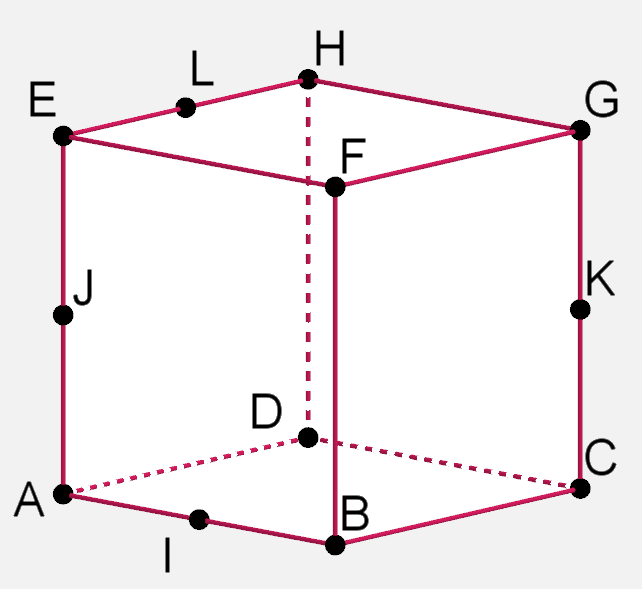
\includegraphics[scale=0.3]{cubecoplan}
\end{center}

D'après la relation de Chasles, $\overrightarrow{AH}=\overrightarrow{AE}+\overrightarrow{EH}$. Or, $J$ étant le milieu de $[AE]$, on a $\overrightarrow{AE}=2\overrightarrow{JE}$. 

De même, $\overrightarrow{EH}=2\overrightarrow{EL}$. Ainsi, $\overrightarrow{AH}=2\overrightarrow{JE}+2\overrightarrow{EL}=2\overrightarrow{JL}$. Les vecteurs $\overrightarrow{AH}$ et $\overrightarrow{JL}$ sont colinéaires.
Les droites $(AH)$ et $(JL)$ sont donc parallèles.

De la même manière, on montre que $\overrightarrow{EB}=2\overrightarrow{JI}$.

On a $\overrightarrow{JK}=\overrightarrow{EG}$ D'après la relation de Chasles, on a donc $\overrightarrow{JK}=\overrightarrow{EH}+\overrightarrow{HC}=\overrightarrow{EH}+\overrightarrow{EB}$. 

En utilisant les points précédents, on a donc que $\overrightarrow{JK}=2\overrightarrow{JL}+2\overrightarrow{JI}$. Les vecteurs $\overrightarrow{JK}$, $\overrightarrow{JI}$ et $\overrightarrow{JL}$ sont donc coplanaires. Les points $I$, $J$, $K$ et $L$ sont donc coplanaires : ces quatre points appartiennent à un même plan.


\begin{center}
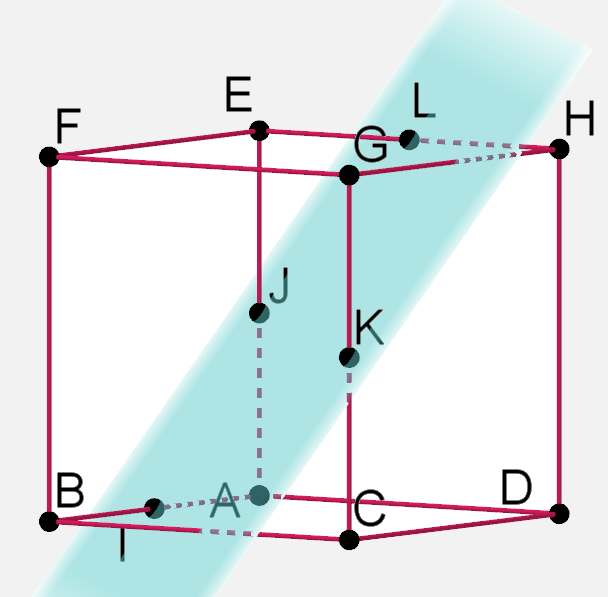
\includegraphics[scale=0.3]{cubecoplan2}
\end{center}

\end{example}
\newpage
\subsection{Positions relatives}

\subsubsection{Positions relatives de deux droites}

\begin{definition} Soit $A$, $B$, $C$ et $D$ quatre points distincts de l'espace. Les droites $(AB)$ et $(CD)$ sont dites coplanaires si les points $A$, $B$, $C$ et $D$ sont coplanaires.

Autrement dit, il existe un plan qui contiennent les droites $(AB)$ et $(CD)$.\end{definition}

\begin{proposition}Deux droites de l'espace coplanaires sont...
\begin{itemize}
\item parallèles ou confondues si leurs vecteurs directeurs sont colinéaires,
\item sécantes en un unique point sinon.
\end{itemize}\end{proposition}


\begin{example}On considère un cube $ABCDEFGH$ ainsi qu'un point $I$ sur le segment $[BF]$.

\begin{minipage}{0.4\linewidth}
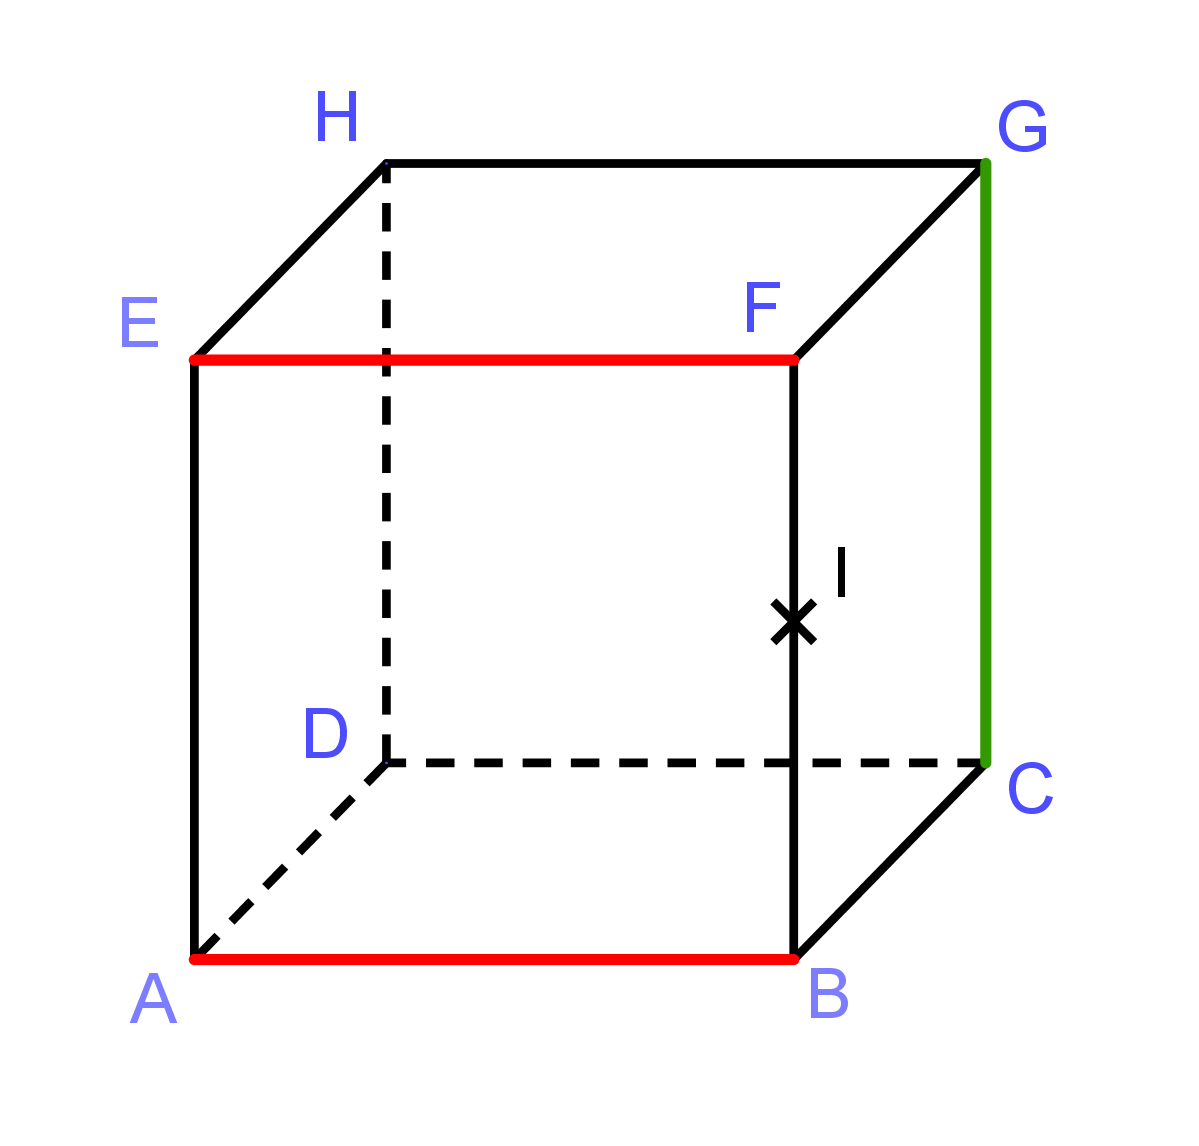
\includegraphics[scale=1.2]{cube1}

\end{minipage}\begin{minipage}{0.6 \linewidth}
\begin{itemize}
\item Les droites $(AB)$ et $(EF)$ sont parallèles.
\item Les droites $(AB)$ et $(CG)$ ne sont pas coplanaires.
\item Les droites $(HI)$ et $(BD)$ sont coplanaires mais pas parallèles : elles sont donc sécantes.
\end{itemize}
\end{minipage}

\end{example}



\subsubsection{Positions relatives d'une droite et d'un plan}

\begin{proposition}Une droite est...
\begin{itemize}
\item parallèle ou contenue dans un plan si tout vecteur de la droite est aussi un vecteur directeur du plan,
\item sécante au plan en un unique point sinon.
\end{itemize}\end{proposition}

\begin{minipage}{0.45\linewidth}\begin{center}
\textbf{Droite sécante à un plan}
\end{center}
\begin{center}
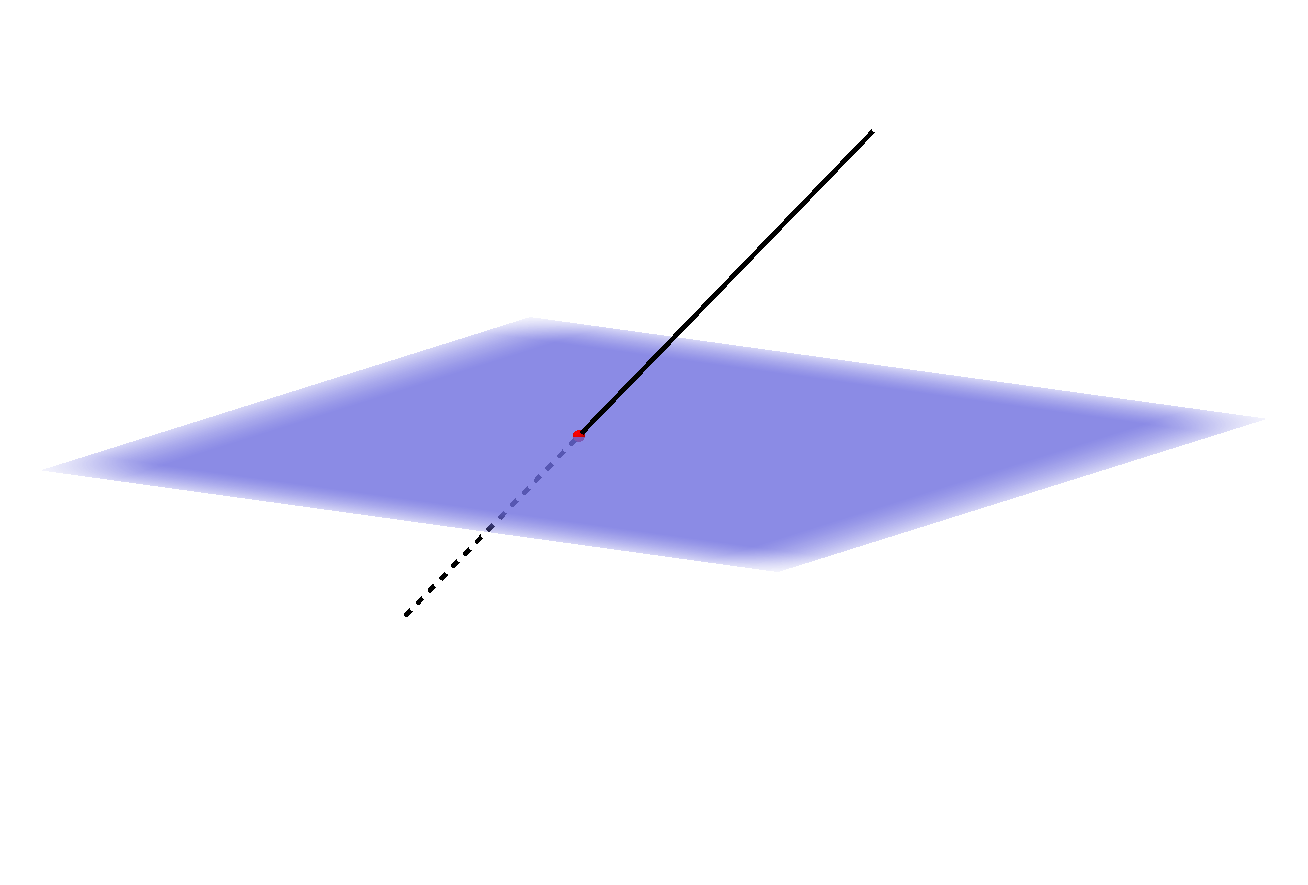
\includegraphics[width=0.8\linewidth]{relatif4}
\end{center}
\end{minipage}\hfill \begin{minipage}{0.45\linewidth}\begin{center}
\textbf{Droite parallèle à un plan}
\end{center}
\begin{center}
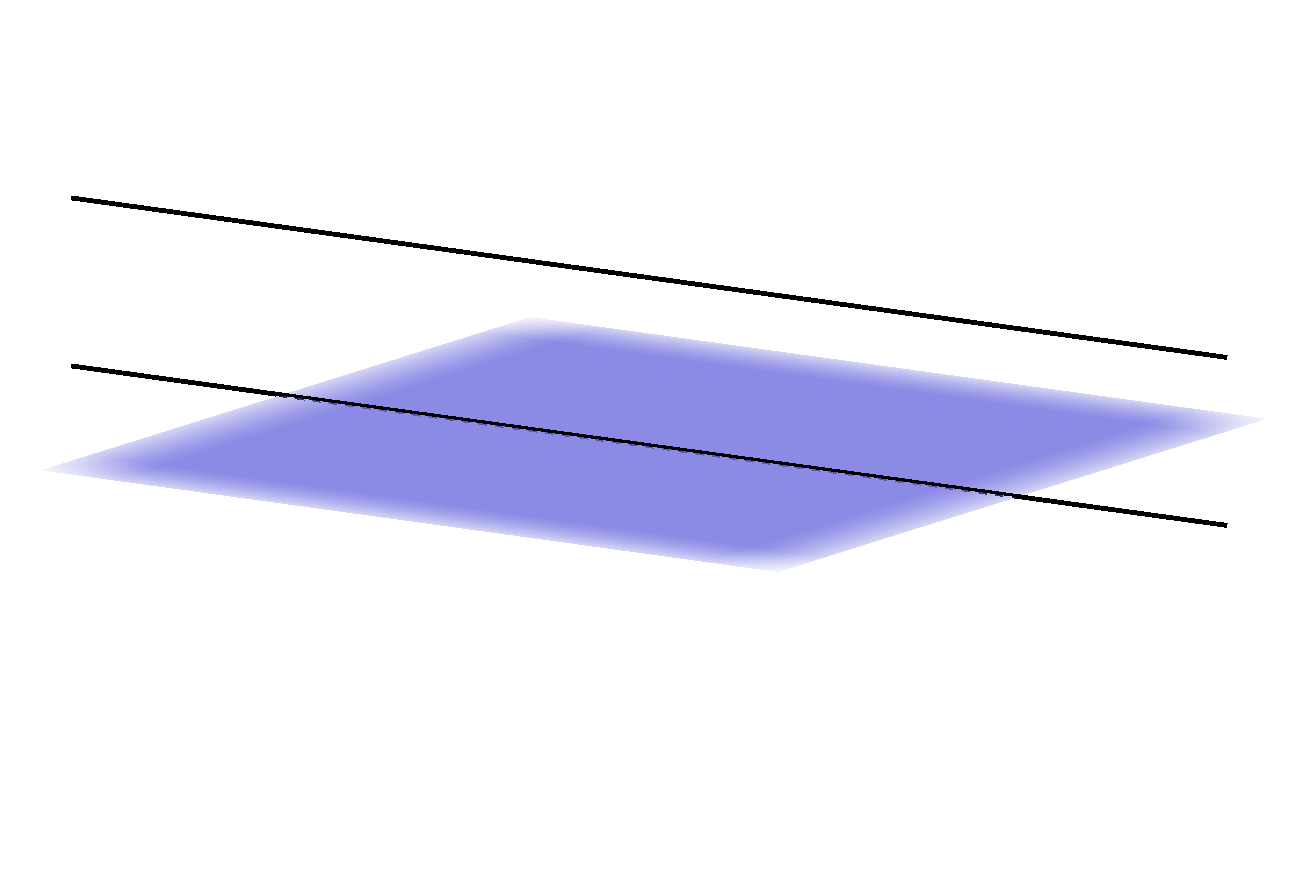
\includegraphics[width=0.8\linewidth]{relatif3}
\end{center}
\end{minipage}

\begin{example}Dans le cube précédent, la droite $(AE)$ est parallèle au plan $(BDH)$. En revanche, cette droite est sécante au plan $(IGH)$.\end{example}

\newpage

\subsubsection{Positions relatives de deux plans}

\begin{proposition}Deux plans de l'espace sont...
\begin{itemize}
\item parallèles ou confondus si les vecteurs directeurs de l'un sont aussi directeurs de l'autre,
\item sécants sinon. L'intersection de ces deux plans est alors une droite.
\end{itemize}\vspace{-0.5cm}\end{proposition}

\begin{minipage}{0.45\linewidth}\begin{center}
\textbf{Plans sécants selon une droite}
\end{center}
\begin{center}
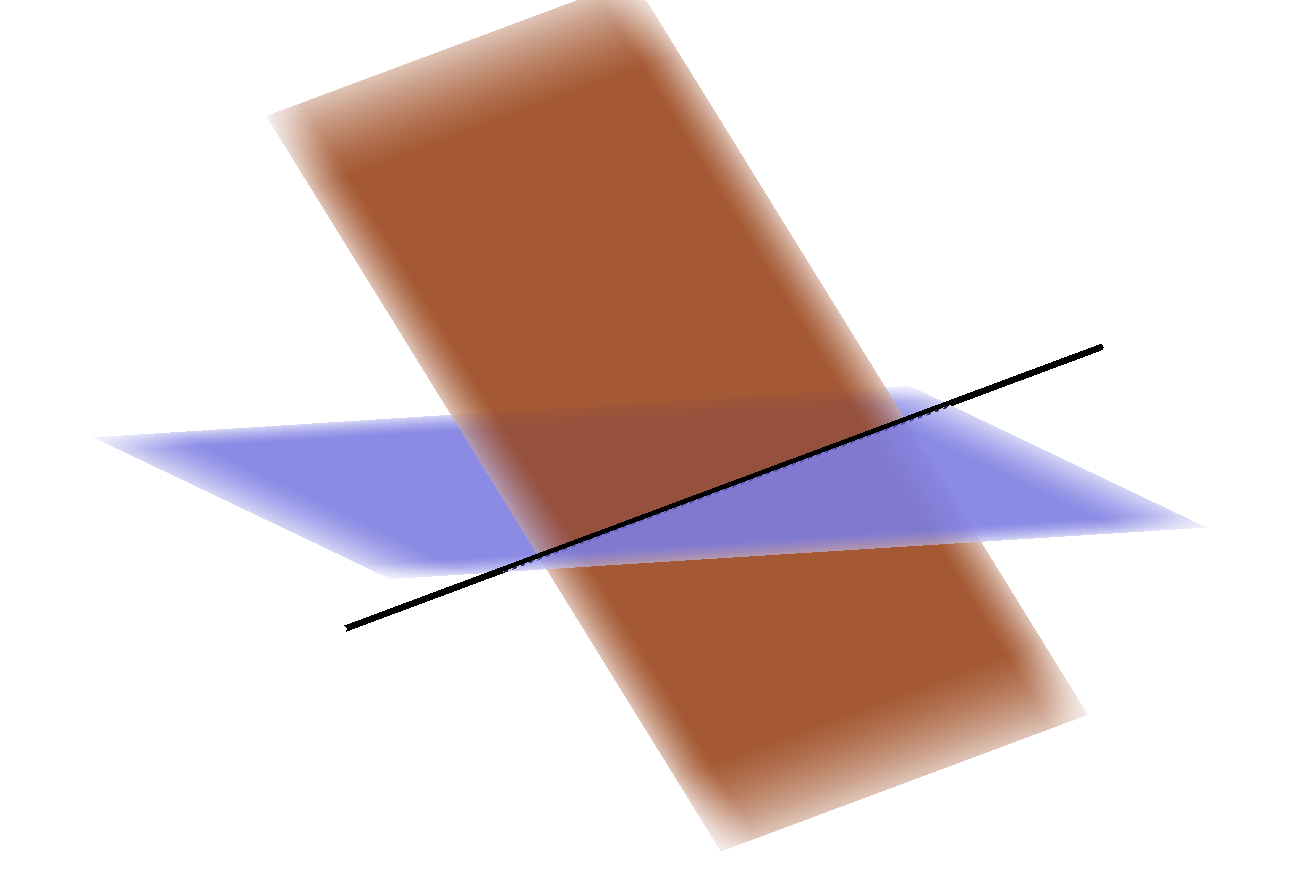
\includegraphics[width=0.7\linewidth]{relatif1}
\end{center}
\end{minipage}\hfill \begin{minipage}{0.45\linewidth}\begin{center}
\textbf{Plans parallèles}
\end{center}
\begin{center}
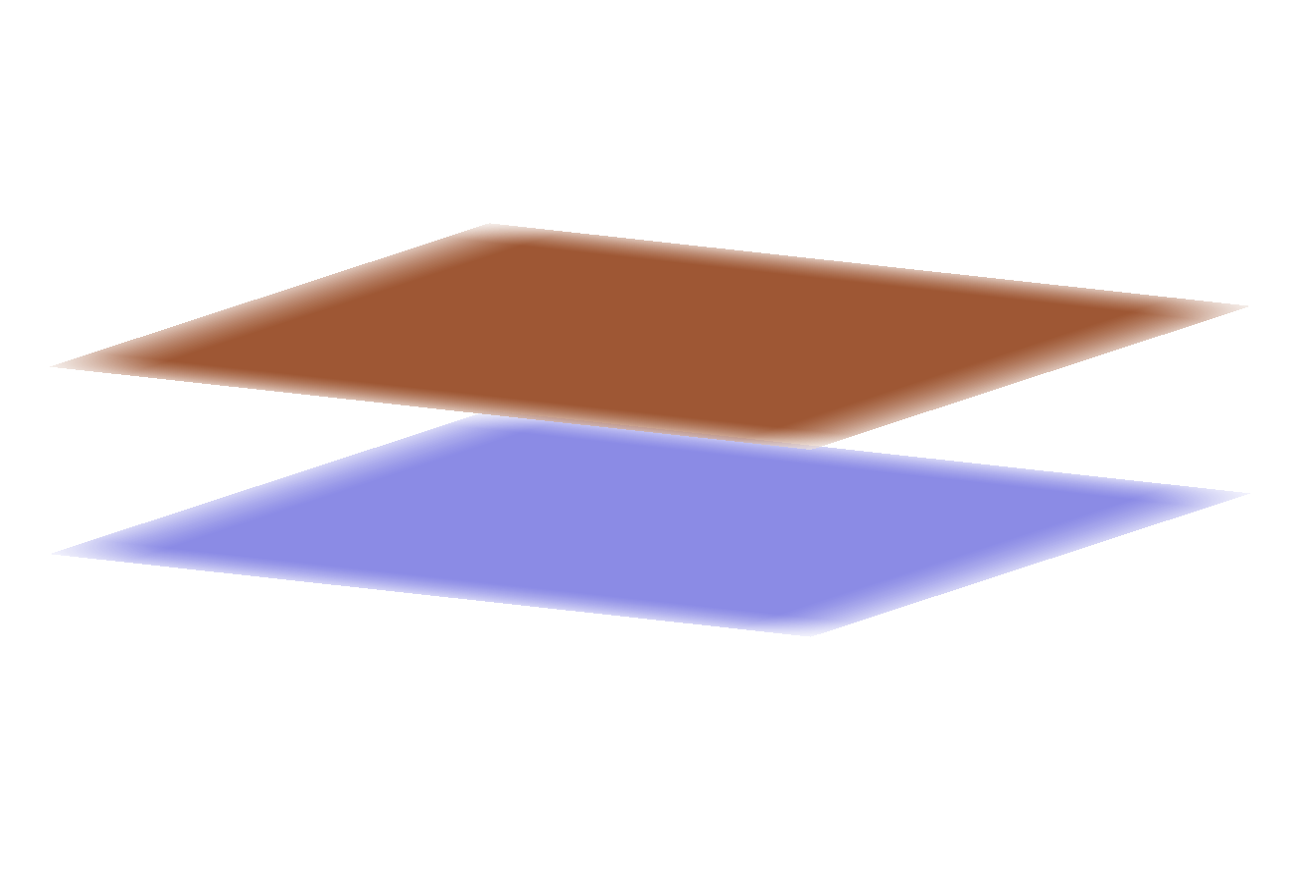
\includegraphics[width=0.7\linewidth]{relatif2}
\end{center}
\end{minipage}

Il suffit donc de connaître deux points d'intersection $A$ et $B$  de deux plans pour déterminer toute leur intersection qui n'est autre que la droite $(AB)$.

\begin{example}On considère le cube $ABCDEFGH$ suivant ainsi que trois points : $I$ sur le segment $[BF]$, $J$ sur le segment $[CG]$ et $K$ sur le segment $[AE]$  de telles sorte que les droites $(IK)$ et $(AB)$ sont sécantes en un point $T$ et que les droites $(IJ)$ et $(BC)$ sont sécantes en un point $S$.

\begin{center}

\includegraphics[scale=0.9]{cube3}
\end{center}


\begin{itemize}
\item Puisque la droite $(IJ)$ est dans le plan $(IJK)$ et la droite $(BC)$ est dans le plan $(ABC)$, le point d'intersection de ces deux droites se trouve dans l'intersection des plans $(ABC)$ et $(IJK)$.
\item Puisque la droite $(IK)$ est dans le plan $(IJK)$ et la droite $(AB)$ est dans le plan $(ABC)$, le point d'intersection de ces deux droites se trouve dans l'intersection des plans $(ABC)$ et $(IJK)$.
\item L'intersection de deux plans sécants étant une droite, l'intersection des plans $(ABC)$ et $(IJK)$ est la droite $(ST)$.
\end{itemize}

\begin{center}
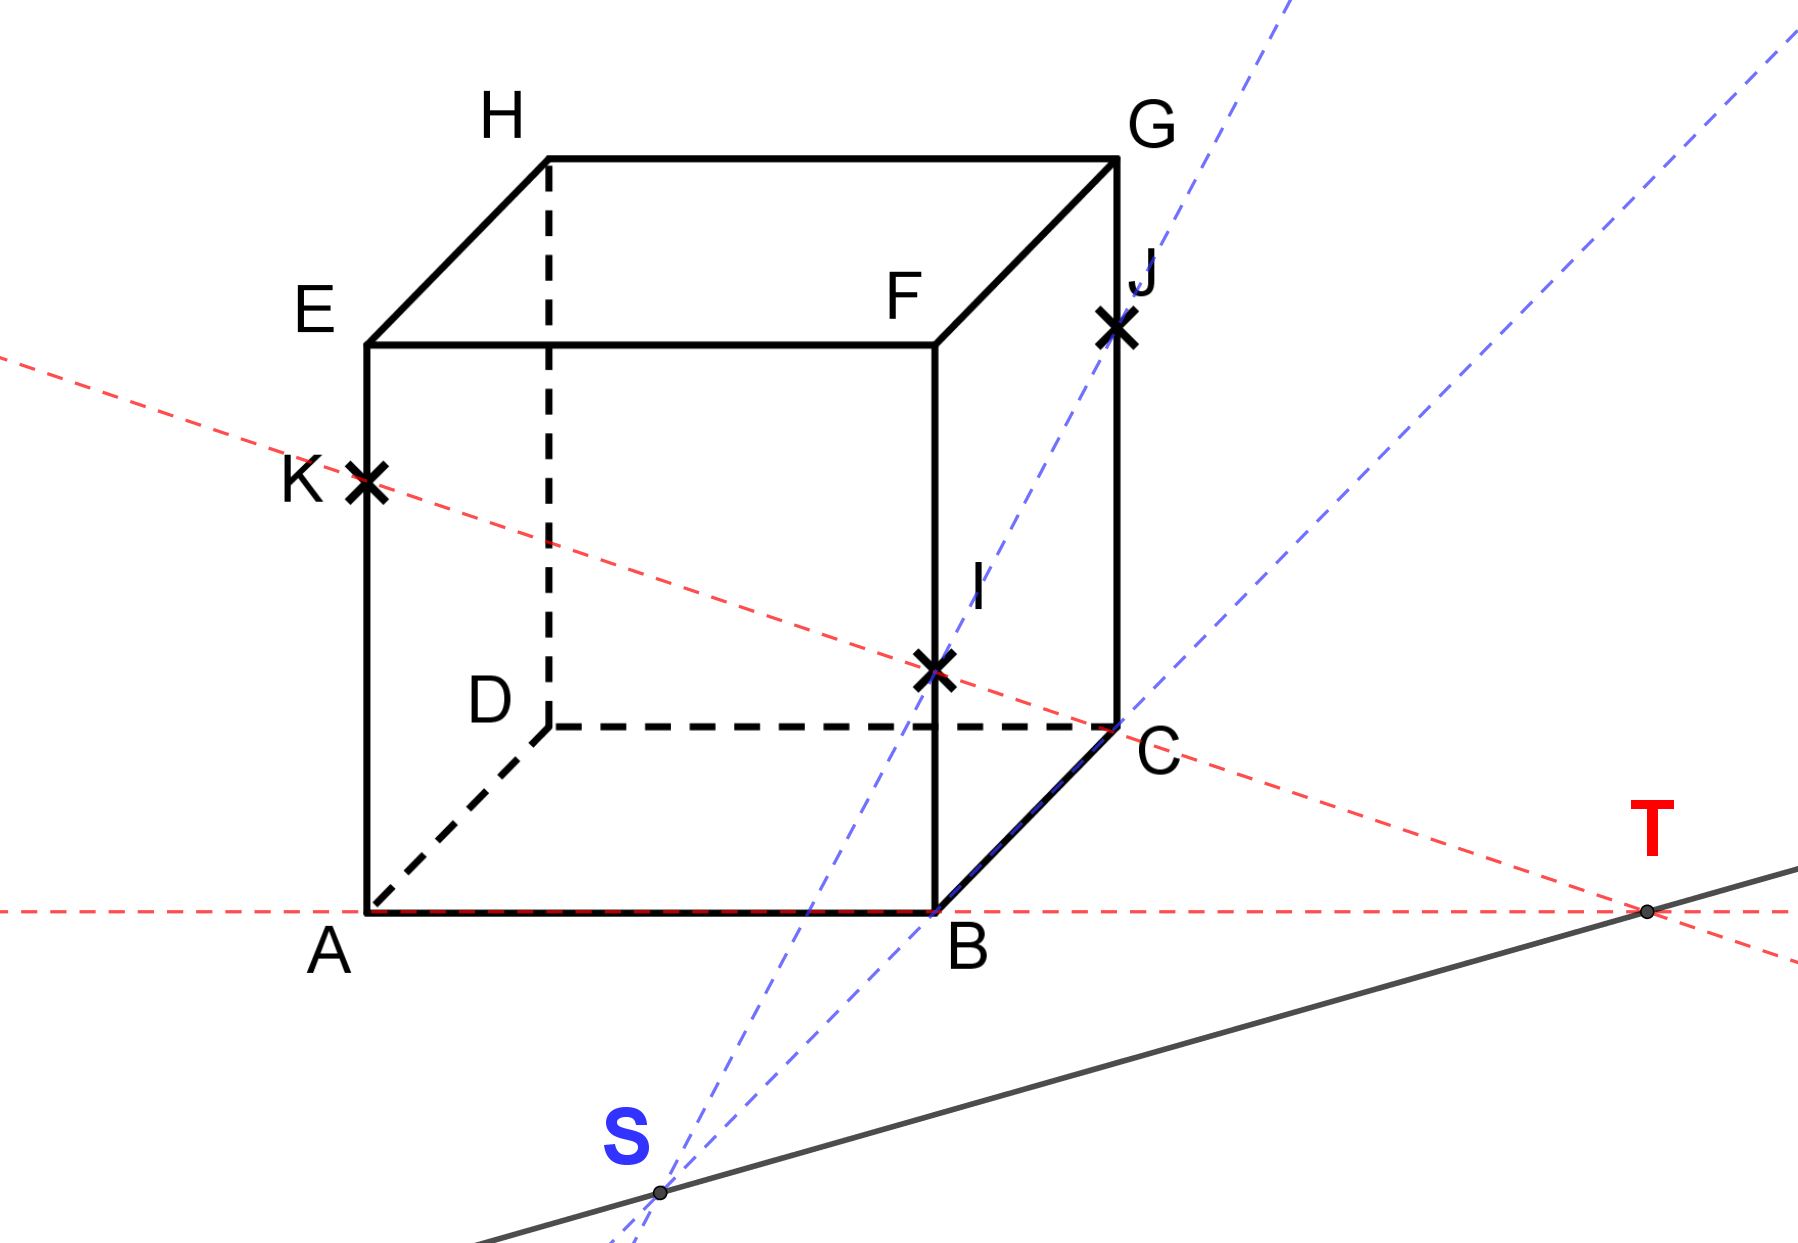
\includegraphics[scale=0.9]{intercube}
\end{center}
 \vspace{-1cm}\end{example}

\begin{proposition}Pour montrer que deux plans $\mathcal{P}$ et $\mathcal{P}'$ sont parallèles, il suffit de trouver deux droites sécantes non confondues $(d_1)$ et $(d_2)$ de $\mathcal{P}$ et deux droites sécantes non confondues $(\delta_1)$ et $(\delta_2)$ de $\mathcal{P}'$ telles que $(d_1)$ est parallèle à $(\delta_1)$ et $(d_2)$ est parallèle à $(\delta_2)$.\end{proposition}

\section{Repère de l'espace}

\begin{definition}Un repère de l'espace est un quadruplet $\Oijk$ où
\begin{itemize}
\item $O$ est un point de l'espace ;
\item $\vec{\imath}$, $\vec {\CMjmath}$ et $\vec k$ sont des vecteurs non coplanaires.
\end{itemize}
On dit que les vecteurs $\vec{\imath}$, $\vec {\CMjmath}$ et $\vec k$ forment une base de l'espace.\end{definition}



\begin{proposition}Soit $\vec u$ un vecteur de l'espace et  $\Oijk$ un repère de l'espace. 

Il existe un unique triplet de réel $(x;y;z)$ tel que $\vec u = x \vec {\imath} + y \vec {\CMjmath} + z \vec k$.

$x$, $y$ et $z$ sont appelés les coordonnées du vecteur $\vec u$. On notera $\vec u\renewcommand{\arraystretch}{1} \renewcommand{\arraystretch}{1}\begin{pmatrix}x\\y\\z\end{pmatrix}$. \end{proposition}

\begin{example}On considère deux cubes $ABCDEFGH$ et $BIJCFLKG$ placés côte à côte.

\begin{center}

\includegraphics[scale=2]{pave2}
\end{center}

Les coordonnées du vecteur $\overrightarrow{AG}$ dans le repère $(A;\overrightarrow{AI}, \overrightarrow{AD}, \overrightarrow{AE})$ sont \renewcommand{\arraystretch}{1}\coordbe{0,5}{1}{ 1 }. 

On a en effet $\overrightarrow{AG}=\dfrac{1}{2}\overrightarrow{AI}+\overrightarrow{AD}+\overrightarrow{AE}.$\end{example}

\begin{definition}Soit $M$ un point de l'espace et $(O;\vec i , \vec j ,\vec k)$ un repère de l'espace. Les coordonnées du point $M$ sont les réels $(x;y;z)$ tels que le vecteur $\overrightarrow{OM}$ a pour coordonnées \renewcommand{\arraystretch}{1}\coordbe{x}{y}{z}. On notera $M(x;y;z)$. \end{definition}

\begin{example}Dans la figure précédente, on a  $\overrightarrow{AK}=\overrightarrow{AB}+\overrightarrow{AC}+\overrightarrow{AE}$ 

Le point $K$ a pour coordonnées $(1,1,1)$ dans le repère $(A;\overrightarrow{AB}, \overrightarrow{AC}, \overrightarrow{AE})$.
\end{example}

\begin{proposition}Dans un repère  $\Oijk$, on considère les points $A(x_A;y_A;z_A)$ et $B(x_B;y_B;z_B)$.
\begin{itemize}
\item Le vecteur $\overrightarrow{AB}$ a pour coordonnées \renewcommand{\arraystretch}{1}\coordbe{x_B-x_A}{y_B-y_A}{z_B-z_A}.
\item Le point $I$, milieu de $[AB]$, a pour coordonnées $\left( \dfrac{x_A+x_B}{2} ; \dfrac{y_A+y_B}{2} ; \dfrac{z_A+z_B}{2} \right)$.
\end{itemize}\end{proposition}

\begin{demonstration}On a $\overrightarrow{OA}=x_A\vec {\imath} + y_A \vec \vec {\CMjmath} + z_A \vec k$ et $\overrightarrow{OB}=x_B\vec \vec {\imath} + y_B \vec {\CMjmath} + z_B \vec k$. Or, d'après la relation de Chasles, $\overrightarrow{AB}=\overrightarrow{AO}+\overrightarrow{OB}=\overrightarrow{OB}- \overrightarrow{OA}$. Ainsi,
\[\overrightarrow{AB} = x_B\vec {\imath} + y_B \vec {\CMjmath} + z_B \vec k - (x_A\vec {\imath} + y_A \vec {\CMjmath} + z_A \vec k)=(x_B-x_A)\vec {\imath} + (y_B-y_A)\vec {\CMjmath} + (z_B - z_A)\vec k.\]
On retrouve bien le résultat attendu. Par ailleurs, si $I(x_I,y_I,z_I)$ est le milieu de $[AB]$, alors $\overrightarrow{AI}=\overrightarrow{IB}$. 

On a donc, en regardant la première coordonnée de ces deux vecteurs, $x_I - x_A = x_B - x_I$ d'où $x_I=\dfrac{x_A+x_B}{2}$. 

En faisant de même avec les deuxièmes et troisièmes coordonnées, on retrouve la formule attendue.\end{demonstration}

\begin{example}On se place dans un repère $\Oijk$. On considère les points $A(1;3;-4)$ et $B(2;7;-1)$. On note $I$ le milieu du segment $[AB]$.
\begin{itemize}
\item Le vecteur $\overrightarrow{AB}$ a pour coordonnées $\renewcommand{\arraystretch}{1}\renewcommand{\arraystretch}{1}\begin{pmatrix}2-1 \\ 7-3 \\ -1-4\end{pmatrix}$ soit $\renewcommand{\arraystretch}{1}\renewcommand{\arraystretch}{1}\begin{pmatrix}1 \\ 4 \\ -5\end{pmatrix}$.
\item Le point $I$ a pour coordonnées $\left( \dfrac{1+2}{2} ; \dfrac{3+7}{2} ; \dfrac{-4+(-1)}{2} \right)$ soit $\left(\dfrac{3}{2};5;-\dfrac{5}{2}\right)$.
\end{itemize}\end{example}

\begin{proposition}Dans un repère  $\Oijk$, on considère les vecteurs $\renewcommand{\arraystretch}{1}\coorde{u}{x}{y}{z}$ et $\renewcommand{\arraystretch}{1}\coorde{v}{x'}{y'}{z'}$. 

Soit $\lambda$ et $\mu$ des réels. Le vecteur $\lambda \vec u + \mu \vec v$ a pour coordonnées \renewcommand{\arraystretch}{1}\coordbe{\lambda x + \mu x'}{\lambda y + \mu y'}{\lambda y + \mu y'}.\end{proposition}

\begin{example}On se place dans un repère de l'espace $\Oijk$. 

Les vecteurs \renewcommand{\arraystretch}{1}\coorde{u}{2}{5}{-3} et \renewcommand{\arraystretch}{1}\coorde{v}{-6}{-15}{9} sont colinéaires. En effet, $\vec v = -3\vec u$.\end{example}

\begin{example} Dans le repère  $\Oijk$, on considère les vecteurs \renewcommand{\arraystretch}{1}\coorde{u}{0}{6}{3} \renewcommand{\arraystretch}{1}\coorde{v}{2}{4}{-7}, \renewcommand{\arraystretch}{1}\coorde{w}{-1}{1}{5} . 

Les vecteurs $\vec u$, $\vec v$ et $\vec w$ sont-ils coplanaires ? D'une part, les vecteurs $\vec v$ et $\vec w$ ne sont pas colinéaires.

Supposons qu'il existe deux réels $\lambda$ et $\mu$ tels que $\vec u = \lambda v + \mu w$. Alors $\renewcommand{\arraystretch}{1}\coordbe{0}{6}{3} = \renewcommand{\arraystretch}{1}\coordbe{2\lambda - \mu}{4\lambda + \mu}{-7\lambda + 5\mu} $.

Nous sommes donc amenés à résoudre le système $\left\{\begin{array}{lll} 2\lambda - \mu & =&0 \\
4 \lambda + \mu &=& 6 \\
-7 \lambda + 5\mu &=& 3 \end{array}\right.$.

\[\left\{\begin{array}{lll} 2\lambda - \mu & =&0 \\
4 \lambda + \mu &=& 6 \\
-7 \lambda + 5\mu &=& 3 \end{array}\right. \Leftrightarrow \left\{\begin{array}{lll} \mu & =& 2\lambda \\
4 \lambda + 2\lambda &=& 6 \\
-7 \lambda + 10\lambda &=& 3 \end{array}\right. \Leftrightarrow \left\{\begin{array}{lll} \mu & =& 2 \lambda \\
6 \lambda &=& 6 \\
3\lambda &=& 3 \end{array}\right. \Leftrightarrow \left\{\begin{array}{lll} \mu & =& 2 \\
\lambda &=& 1 \\
\lambda &=& 1 \end{array}\right.\]

Le fait d'avoir deux fois la même ligne n'est pas anormal : nous avons trois équations pour deux inconnues. Si les résultats de ces deux lignes sont différents, cela signifie que les vecteurs ne sont pas coplanaires.

\textbf{Vérifions que les valeurs trouvées pour $\lambda$ et $\mu$ conviennent.}

Les coordonnées de $\vec v + 2 \vec w$ sont en effet \renewcommand{\arraystretch}{1}\coordbe{2 + 2 \times (-1)}{4 + 2 \times 1}{-7 + 2 \times 5} soit \renewcommand{\arraystretch}{1}\coordbe{0}{6}{3}. 

On a donc $\vec u = \vec{v} + 2 \vec w$. Les vecteurs $\vec u$, $\vec v$ et $\vec w$ sont donc coplanaires.

\end{example}


\section{Représentation paramétrique de droite}

\begin{proposition}L'espace est muni d'un repère $\Oijk$.

Soit $A (x_A,y_A,z_A)$ un point de l'espace et $\renewcommand{\arraystretch}{1}\coorde{u}{a}{b}{c}$ un vecteur non nul de l'espace.

On note $(d)$ la droite passant par le point $A$ et dirigée par $\vec u$.

Un point $M(x,y,z)$ appartient à la droite $(d)$ si et seulement s'il existe un réel $t$ tel que $\renewcommand{\arraystretch}{1}\left\{ \begin{array}{l}x=x_A+ta \\ y=y_A+tb \\ z = z_A + tc \\

\end{array}\right.$.
\end{proposition}

\begin{demonstration} Le point $M$ appartient à la droite $(d)$ si et seulement si les vecteurs $\overrightarrow{AM}$ et $\vec u$ sont colinéaires. Puisque $\vec u$ est non nul, cela revient à dire qu'il existe un réel $t$ tel que $\overrightarrow{AM}=t \vec u$.


Ainsi, \renewcommand{\arraystretch}{1}\coordbe{x-x_A}{y-y_A}{z-z_A} = \renewcommand{\arraystretch}{1}\coordbe{ta}{tb}{tc} ou encore $\left\{ \begin{array}{l}x=x_A+ta \\ y=y_A+tb \\ z = z_A + tc \\

\end{array}\right.$.\end{demonstration}

\begin{definition}Soit $A (x_A,y_A,z_A)$ un point de l'espace, $\renewcommand{\arraystretch}{1}\coorde{u}{a}{b}{c}$ un vecteur non nul de l'espace et $(d)$ la droite passant par le point $A$ et dirigée par $\vec u$.

Le système $ \left\{ \renewcommand{\arraystretch}{1}\begin{array}{l}x=x_A+ta \\ y=y_A+tb \\ z = z_A + tc \\

\end{array}\right.,\,t\in\mathbb{R}$ est appelé représentation paramétrique de la droite $(d)$.

\end{definition}

\textbf{Attention ! Une représentation paramétrique de droite n'est pas unique !}

\begin{example} La droite passant par le point $A(2;1;3)$ et dirigée par le vecteur \renewcommand{\arraystretch}{1}\coorde{u}{1}{-3}{2} admet pour représentation paramétrique $\left\{ \renewcommand{\arraystretch}{1}\begin{array}{l}x=2+t \\ y=1-3t \\ z = 3+2t \\

\end{array}\right., t \in \mathbb{R}$.\end{example}

\begin{example}On considère la droite admettant pour représentation paramétrique $ \left\{\renewcommand{\arraystretch}{1} \begin{array}{l}x=5-2t \\ y=8-4t \\ z =3+t \\

\end{array}\right., t \in \mathbb{R}$.
Cette droite passe par le point $A(5,8,3)$ et est dirigée par le vecteur \renewcommand{\arraystretch}{1}\coorde{u}{-2}{-4}{1}.
En prenant $t=2$, on obtient que cette droite passe par le point de coordonnées $(1,0,5)$.

Le point $B(-1;-4;5)$ appartient-il à cette droite ? 

Supposons que ce soit le cas. Il existe alors un réel $t$ tel que $5-2t=-1$, $8-4t=-4$ et $3+t=5$. 

La résolution de ces équations donne successivement $t=3$, $t=3$ et $t=2$. 

Il n'y a pas une unique valeur de $t$ qui est trouvée : le point $B$ n'appartient donc pas à la droite considérée.\end{example}

\begin{example}On considère les droites $(d)\,:\,\left\{ \renewcommand{\arraystretch}{1}\begin{array}{l}x=4-t \\ y=11-3t \\ z = 9-2t \\
\end{array}\right.,\, t \in \mathbb{R}$ et $(d')\,:\,\left\{ \renewcommand{\arraystretch}{1}\begin{array}{l}x=2+k \\ y=6+4k \\ z = -2-5k \\
\end{array}\right.,\, k \in \mathbb{R}$.

On souhaite déterminer, s'il existe, le point d'intersection de ces droites. Il faut donc trouver deux paramètres $t$ et $k$ qui correspondent à un même point pour ces deux droites. Cela nous amène à résoudre le système suivant :

\[\left\{\renewcommand{\arraystretch}{1}\begin{array}{l}4-t=2+k \\ 11-3t=6+4k \\ 9-2t=-2-5k \\\end{array}\right. \Leftrightarrow \left\{\renewcommand{\arraystretch}{1}\begin{array}{l}2-t=k \\ 11-3t=6+4(2-t) \\ 9-2t=-2-5(2-t) \\\end{array}\right. \Leftrightarrow \left\{\renewcommand{\arraystretch}{1}\begin{array}{l}2-t=k \\ 11-3t=6+8-4t \\ 9-2t=-2-10+5t \\\end{array}\right.\]
\[  \Leftrightarrow \left\{\renewcommand{\arraystretch}{1}\begin{array}{l}2-t=k \\ t=3 \\ t=3 \\\end{array}\right.\Leftrightarrow \left\{\renewcommand{\arraystretch}{1}\begin{array}{l}k=2-3=-1 \\ t=3  \\\end{array}\right. .\]

La solution que l'on trouve est unique, les droites sont donc sécantes en un point. Pour trouver les coordonnées de ce point, on remplace le paramètre $t$ ou $k$ dans la représentation paramétrique de la droite correspondante (le mieux étant de le faire pour les deux pour contrôler nos calculs).

En prenant $t=3$ dans la représentation paramétrique de $(d)$, on obtient le point de coordonnées $(1;2;3)$. De même, en prenant $k=-1$ dans la représentation paramétrique de $(d')$, on aboutit également au point de coordonnées $(1;2;3)$. Ce point est le point d'intersection des droites $(d)$ et $(d')$.
\end{example}


\end{document}